\chapter{Configuración red LAN}\label{ch:red lan}

		\section{Definición de una red LAN}
		Una red de área local (LAN) es un conjunto de dispositivos, como impresoras, sistemas informáticos, dispositivos móviles y consolas de juegos, que están interconectados mediante alguna tecnología y comparten datos entre sí. Una LAN puede funcionar como una entidad autónoma e independiente o formar parte de redes más grandes y extensas.
		
		\section{Significado de una dirección IP}
		Una dirección IP (Protocolo de Internet, correspondiente al nivel de red del modelo TCP/IP) es un número que identifica de manera lógica y jerárquica una interfaz de red de un dispositivo. En un paquete IP, el encabezado contiene una dirección de 32 bits (IPv4) o 128 bits (IPv6). Este identificador es único y no se repite en ningún otro equipo en el mundo, y tiene la función de registrar el equipo en la red global. Las direcciones IP no solo son asignadas a equipos de cómputo, sino también a módems, routers, sitios web, entre otros.
		
		En el mundo del direccionamiento IP, se distinguen dos tipos de direcciones IP: dinámicas y estáticas.
		\begin{itemize}
			\item Las direcciones IP dinámicas son variables y son entregadas y administradas por un servidor DHCP. Su funcionamiento se basa en el arrendamiento de la dirección por un tiempo específico, tras el cual la dirección se renovará y puede cambiar su sintaxis.
		
			\item Las direcciones IP estáticas, como su nombre indica, son direcciones fijas que no cambian. Se utilizan en servidores, máquinas de producción conectadas a la red y, en general, por usuarios que no necesitan que su dirección IP varíe, ya que otros servicios dependen de ellas.
		\end{itemize}
			
		\section{Configuración de red}
		
		Para mantener la simplicidad en la red del aula, se ha decidido asignar direcciones IP dinámicas a los ordenadores de escritorio. Sin embargo, el servidor de virtualización recibirá una dirección IP estática para que las estaciones de trabajo puedan localizarlo en la red.
		
		La red del aula utilizará la dirección IP 192.168.1.0/24 y se ha establecido la dirección IP 192.168.1.222 para el servidor de virtualización.
				
		\subsection{Diagrama de red}
				
			El diagrama de red es una representación visual que muestra los ordenadores que formarán parte de la red de trabajo y su interconexión.\par
			
			\begin{figure}[h]
				\centering
				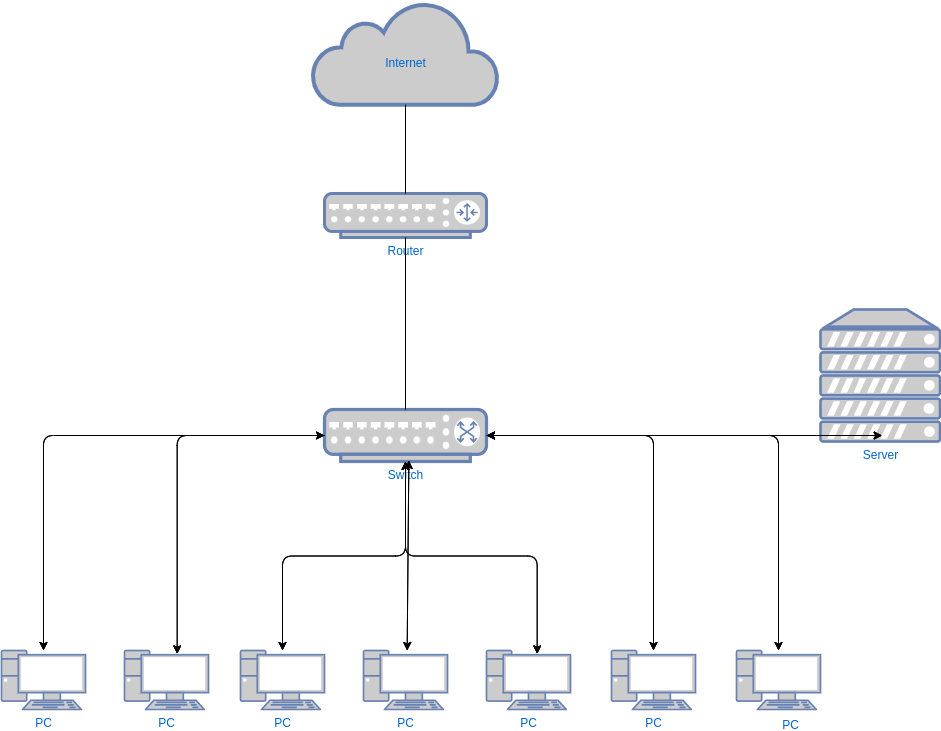
\includegraphics[height=0.6\textwidth]{imagenes/red/diagrama.png}
				\caption{Diagrama de red}
				\label{fig:red local lan}
			\end{figure}
			
				
